\usetikzlibrary{shapes.geometric, arrows,arrows.meta,matrix}

% Blocks
\tikzstyle{floating} = [text centered]
\tikzstyle{coltitle} = [anchor=west]
\tikzstyle{mintitle} = [anchor=west,font=\scriptsize]
\tikzstyle{label} = [text centered, font=\bfseries]
\tikzstyle{clf} = [rectangle, rounded corners, text centered, draw=black]
\tikzstyle{q} = [circle, text centered, draw=black]

% Arrows
\tikzstyle{dependency} = [thick, -{Latex[round,open]}, dash pattern= on 1pt off 1pt]
\tikzstyle{flow} = [thick, ->]


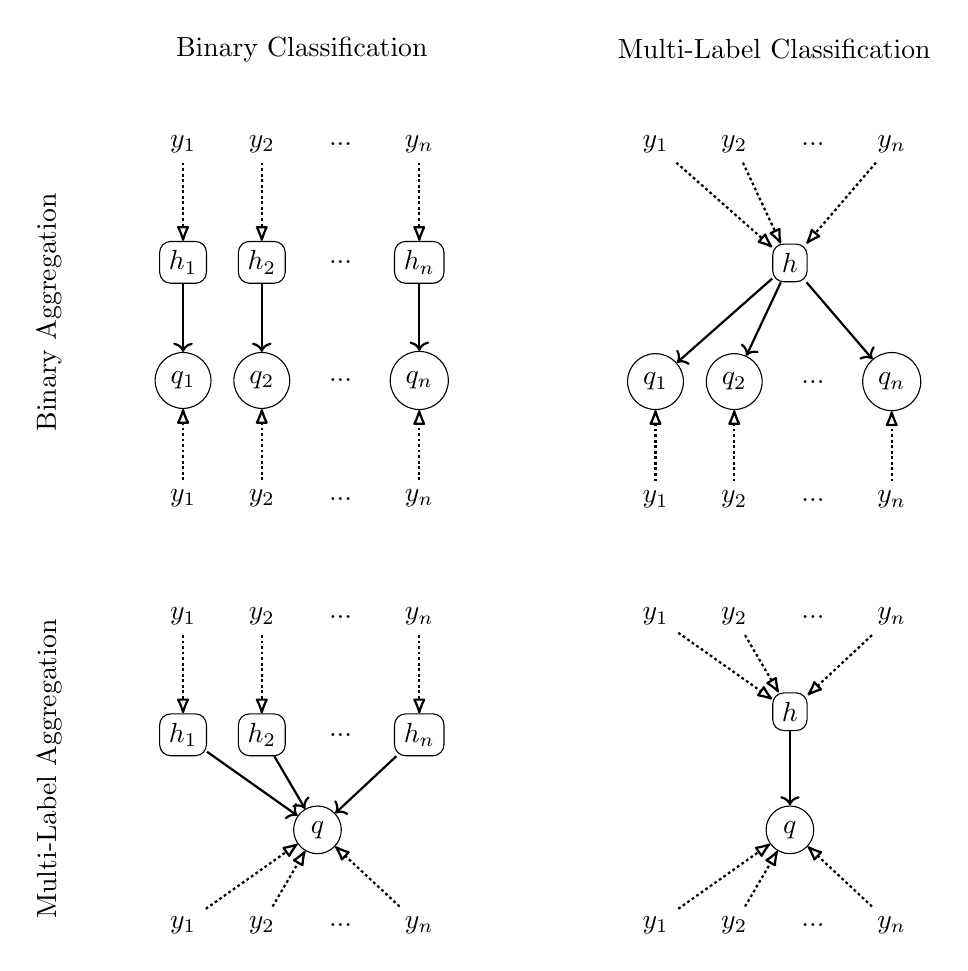
\begin{tikzpicture}
	% NAIVE
	\node(y1_top)[label]{$y_1$};
	\node(y2)[label, right of=y1_top]{$y_2$};
    \node(hdots)[floating, right of=y2]{...};
	\node(yn_top)[label, right of=hdots]{$y_n$};

    \node(h1)[clf, below of=y1_top, yshift=-5mm]{$h_1$};
    \node(h2)[clf, right of=h1]{$h_2$};
    \node(hdots)[floating, right of=h2]{...};
    \node(hn)[clf, right of=hdots]{$h_n$};

	\draw [dependency] (y1_top) -- (h1);
	\draw [dependency] (y2) -- (h2);
	\draw [dependency] (yn_top) -- (hn);

	\node(q1)[q, below of=h1, yshift=-5mm]{$q_1$};
	\node(q2)[q, right of=q1]{$q_2$};
	\node(hdots)[floating, right of=q2]{...};
	\node(qn)[q, right of=hdots]{$q_n$};

	\draw [flow] (h1) -- (q1);
	\draw [flow] (h2) -- (q2);
	\draw [flow] (hn) -- (qn);

	\node(y1_bot)[label, below of=q1, yshift=-5mm]{$y_1$};
	\node(y2)[label, right of=y1_bot]{$y_2$};
    \node(hdots)[floating, right of=y2]{...};
	\node(yn)[label, right of=hdots]{$y_n$};

	\draw [dependency] (y1_bot) -- (q1);
	\draw [dependency] (y2) -- (q2);
	\draw [dependency] (yn) -- (qn);


	%BQMC
	\node(y1_top2)[label, right of=yn_top,xshift=2cm]{$y_1$};
	\node(y2)[label, right of=y1_top2]{$y_2$};
    \node(hdots)[floating, right of=y2]{...};
	\node(yn)[label, right of=hdots]{$y_n$};

    \node(h)[clf, below right of=y2, yshift=-8mm]{$h$};

	\draw [dependency] (y1_top2) -- (h);
	\draw [dependency] (y2) -- (h);
	\draw [dependency] (yn) -- (h);

	\node(q2)[q, below left of=h, yshift=-8mm]{$q_2$};
	\node(q1)[q, left of=q2]{$q_1$};
	\node(hdots)[floating, right of=q2]{...};
	\node(qn)[q, right of=hdots]{$q_n$};

	\draw [flow] (h) -- (q1);
	\draw [flow] (h) -- (q2);
	\draw [flow] (h) -- (qn);

	\node(y1)[label, below of=q1, yshift=-5mm]{$y_1$};
	\node(y2)[label, right of=y1]{$y_2$};
    \node(hdots)[floating, right of=y2]{...};
	\node(yn)[label, right of=hdots]{$y_n$};

	\draw [dependency] (y1) -- (q1);
	\draw [dependency] (y2) -- (q2);
	\draw [dependency] (yn) -- (qn);

	% MQBC
	\node(y1_top3)[label, below of=y1_bot,yshift=-5mm]{$y_1$};
	\node(y2)[label, right of=y1_top3]{$y_2$};
    \node(hdots)[floating, right of=y2]{...};
	\node(yn_top)[label, right of=hdots]{$y_n$};

    \node(h1)[clf, below of=y1_top3, yshift=-5mm]{$h_1$};
    \node(h2)[clf, right of=h1]{$h_2$};
    \node(hdots)[floating, right of=h2]{...};
    \node(hn)[clf, right of=hdots]{$h_n$};

	\draw [dependency] (y1_top3) -- (h1);
	\draw [dependency] (y2) -- (h2);
	\draw [dependency] (yn_top) -- (hn);

	\node(q)[q, below right of=h2, yshift=-5mm]{$q$};

	\draw [flow] (h1) -- (q);
	\draw [flow] (h2) -- (q);
	\draw [flow] (hn) -- (q);

	\node(y2)[label, below left of=q, yshift=-5mm]{$y_2$};
	\node(y1)[label, left of=y2]{$y_1$};
    \node(hdots)[floating, right of=y2]{...};
	\node(yn)[label, right of=hdots]{$y_n$};

	\draw [dependency] (y1) -- (q);
	\draw [dependency] (y2) -- (q);
	\draw [dependency] (yn) -- (q);

	% MQMC
	\node(y1_top4)[label, right of=yn_top,xshift=2cm]{$y_1$};
	\node(y2)[label, right of=y1_top4]{$y_2$};
    \node(hdots)[floating, right of=y2]{...};
	\node(yn)[label, right of=hdots]{$y_n$};

    \node(h)[clf, below right of=y2, yshift=-5mm]{$h$};

	\draw [dependency] (y1_top4) -- (h);
	\draw [dependency] (y2) -- (h);
	\draw [dependency] (yn) -- (h);

	\node(q)[q, below of=h, yshift=-5mm]{$q$};

	\draw [flow] (h) -- (q);

	\node(y2)[label, below left of=q, yshift=-5mm]{$y_2$};
	\node(y1)[label, left of=y2]{$y_1$};
    \node(hdots)[floating, right of=y2]{...};
	\node(yn)[label, right of=hdots]{$y_n$};

	\draw [dependency] (y1) -- (q);
	\draw [dependency] (y2) -- (q);
	\draw [dependency] (yn) -- (q);

	\node(bc)[coltitle,above right of=y1_top,xshift=8mm,yshift=5mm]{Binary Classification};
	\node(mc)[coltitle, right of=bc, xshift=50mm]{Multi-Label Classification};
	\node(bq)[coltitle,rotate=90, above left of=bc,anchor=east,xshift=-10mm,yshift=25mm]{Binary Aggregation};
	\node(mq)[coltitle, rotate=90, anchor=east, left of=bq, xshift=-48mm]{Multi-Label Aggregation};

	\node(bqbc)[mintitle,above of=y1_top,xshift=15mm,yshift=-5mm]{\bqbc};
	\node(bqmc)[mintitle,above of=y1_top2,xshift=15mm,yshift=-5mm]{\bqmc};
	\node(mqbc)[mintitle,above of=y1_top3,xshift=15mm,yshift=-5mm]{\mqbc};
	\node(mqmc)[mintitle,above of=y1_top4,xshift=15mm,yshift=-5mm]{\mqmc};
\end{tikzpicture}
